\documentclass[10pt]{article}
\usepackage[a4paper,margin=1.7cm]{geometry}
\usepackage[T1]{fontenc}
\usepackage{lmodern}
\usepackage{microtype}
\usepackage{booktabs}
\usepackage{graphicx}
\usepackage{amsmath}
\usepackage{xcolor}
\usepackage[hidelinks]{hyperref}
\usepackage{enumitem}
\usepackage{caption}
\setlist{nosep,leftmargin=1.2em}
\setlength{\parskip}{3pt}
\setlength{\parindent}{0pt}
\captionsetup{font=small}
\newcommand{\pp}{\,pp}
\newcommand{\todo}[1]{\textcolor{red}{[#1]}}
\graphicspath{{../../results/figures/}}

\begin{document}

{\large\bfseries DeepVoice: Do Fake-Voice Detectors Learn Fakeness, or Just the Dataset?}\\[2pt]
Progress report \textbullet{} Hashem Awad, Ahmed Faleh, Ali Sleiman \textbullet{} CMPS 261, Dr.\ Aya Kayal \textbullet{} 6 November 2026

\section*{1\quad Problem statement and changes since the proposal}
We ask \emph{what fake-voice detectors learn, and how much of their performance survives when the data
changes}. We train detectors of increasing complexity on ASVspoof 2019 LA, test them on unseen attacks
and on a new data source, and check for shortcuts, trustworthy confidence, and whether the large
pretrained model is worth its cost. Following the feedback, we \textbf{narrowed the scope}: five core
experiments (E1 model ladder, E2 features, E3 tuning/overfitting, E4 generalization, E5 shortcuts,
calibration and failure analysis), three core detectors plus a silence-only control, and four
hypotheses. \textbf{We no longer build our own English/Arabic test set}: we cannot separate language
from recording conditions and generator quality, so it is an optional extension reported
descriptively. The ``new data'' test now uses the existing \textbf{In-the-Wild} (ITW) corpus.
Hypotheses H1--H4 (silence shortcut; unseen attacks harder; pretrained model wins in-distribution with
a shrinking edge; dev thresholds fail on ITW) were written with numeric decision rules and frozen
(sha256 \texttt{9494fc18\ldots b76b}, committed) \emph{before} any eval or ITW run.

\section*{2\quad Data and preprocessing}
\textbf{ASVspoof 2019 LA} (official splits, verified against the protocol files): train 2,580 real +
22,800 fake (20 speakers), dev 2,548 + 22,296 (20), eval 7,355 + 63,882 (67); about 90\% fake;
speakers do not overlap. Train/dev use attacks A01--A06; eval uses A07--A19, of which A16 and A19 reuse
the algorithms of A04 and A06 [1], leaving \textbf{11 truly unseen attacks}.
\textbf{In-the-Wild} [2]: 19,963 real + 11,816 fake clips (37.9\,h) from \textbf{54} public figures
(not 58 as often quoted); every speaker has both classes. \textbf{Preprocessing}: one loader for both
corpora (16\,kHz mono); clip lists come from protocol files only. Features are computed once and
cached: \textbf{S} silence/duration/energy from an energy VAD (25\,ms frames; speech = within 35\,dB of
the clip's peak), \textbf{M} MFCC and \textbf{L} LFCC (40 coefficients + $\Delta$ + $\Delta\Delta$),
\textbf{P} six spectral descriptors; frame values are pooled over time (mean, std, min, max,
percentiles), and smaller settings for ablations are column subsets. \textbf{XLS-R-300M} embeddings
(mean-pooled, every 3rd layer) are extracted once for all clips on the laptop GPU (64\,ms/clip).
\textbf{Audit} (Fig.~1): real clips start speaking later (median leading silence 0.88\,s vs 0.39\,s),
driven by attacks A01, A03, A04; duration, trailing silence and loudness barely differ.

\section*{3\quad Evaluation metrics}
The primary metric is the \textbf{equal error rate (EER)}: the error at the threshold where the share
of real clips called fake equals the share of fakes called real (50\% = guessing). It is
threshold-free and insensitive to the 90/10 class imbalance, where accuracy is misleading (always
answering ``fake'' scores 90\%); it is also the ASVspoof standard. For models with few distinct scores
we interpolate between ROC points. Clips from one speaker are correlated, so every EER has a
\textbf{speaker-clustered bootstrap 95\% CI} (1,000 resamples of whole speakers). For E5 we add the
expected calibration error (ECE, 15 bins) and the error at the dev-chosen threshold (H4); every rung
also reports training time, latency and size. Models are fit on train, selected on dev, and scored on
eval once per final model.

\section*{4\quad Classical baseline}
\textbf{Rung 0} (four silence/duration numbers; logistic regression and a depth-3 tree) reaches
28.0\% dev EER. Scored once on eval, the tree reaches \textbf{19.1\%} [18.6, 19.5]: below the 25\% bar,
so \textbf{H1a is supported}, consistent with [5]. Per attack (Fig.~2a) it catches 10 of 13 eval attacks at 1--11\% EER
without hearing the voice, and is at chance only on A17--A19. \textbf{Rung 1} (Fig.~3): LFCC dominates;
dropping it raises dev EER from about 0.5--1\% to 6--9\%, while dropping S, M or P barely matters.
More coefficients and deltas help (LFCC random forest: 3.3\% with 13, 1.4\% with 20, 0.49\% with 40
coefficients); MFCC stays above 8\%. We then tuned logistic regression (LR), random forest (RF) and
gradient boosting (HGB) on LFCC-40+$\Delta$+$\Delta\Delta$ by random search (30 settings each),
selected on dev and, separately, by speaker-grouped 5-fold CV on train (Fig.~4):

\begin{center}\small
\begin{tabular}{lccccc}
\toprule
Model (LFCC-40) & Untuned dev & Tuned dev [95\% CI] & Grouped CV & Train & Dev EER of CV's pick \\
\midrule
Logistic regression & 0.60 & 0.48 [0.20, 0.89] & 2.43 & 0.04 & 1.16 (different pick) \\
Random forest & 0.49 & 0.43 [0.19, 0.85] & 1.54 & 0.00 & 0.48 (different pick) \\
Gradient boosting & 0.31 & \textbf{0.13} [0.04, 0.25] & 0.90 & 0.00 & same pick \\
\bottomrule
\end{tabular}
\end{center}
(EER in \%.) Tuning helps modestly; gradient boosting is best and keeps improving with more data,
while LR and RF flatten from 25\% of train (Fig.~4a). All models fit train almost perfectly, and
grouped-CV EER is 2--7$\times$ the dev EER, so selection is sensitive to which speakers are held out;
CV and dev agree only for gradient boosting. \textbf{Final rung 1 on eval} (tuned gradient boosting,
scored once): \textbf{14.1\%} [12.8, 15.5], about 100$\times$ its dev EER and only 5\pp{} better than
silence alone. It stays near-perfect on the repeated attacks (A16, A19: 0.2--0.3\%) but fails on unseen
A17 and A18 (36--38\%), so H2's rule (worst unseen $\geq 2\times$ repeated) is met.

\section*{5\quad Sophisticated model: frozen XLS-R-300M}
XLS-R-300M [3] is a 300M-parameter speech transformer pretrained without labels on about 436k hours in
128 languages. Kept frozen, it turns each clip into one 1,024-number vector per layer; a logistic
regression on top is the detector. We expect it to beat hand-made features because its layers encode
fine acoustic detail learned from far more speech, and self-supervised features are reported to
generalize better to unseen spoofing systems [4]. \textbf{Progress}: embeddings are extracted for all
ASVspoof clips (train, dev, eval; 2\,h on the laptop GPU); ITW is running. \textbf{Preliminary results} (Fig.~2b): early
layers are best, with dev EER 0.00\% [0.00, 0.02] at layer 3 and 0.01\% at layer 6, against 0.49\% for
the best untuned classical model. Dev is now saturated, because it repeats the training attacks; eval
(H3 requires a margin of at least 5\pp) is the real test. Cost so far: 64\,ms/clip extraction on the
laptop GPU vs 23\,ms/clip for LFCC on one CPU core; the classifier trains in under 1\,s.

\section*{6\quad Remaining plan and risks (to 20 November)}
\textbf{Nov 7--8}: finish E1 (rung 2 on eval, cost table), XLS-R layer choice and small MLP on dev.
\textbf{Nov 9--10}: E4: per-attack EER for every rung (H2), ITW for every rung including rung 0 as a
shortcut control (H3, H4). \textbf{Nov 11--12}: E5: trim silence and change loudness at test time
(H1b), retrain with silence/gain augmentation, calibration (reliability diagrams, ECE, temperature
scaling), failure analysis by attack, duration, silence and speaker. \textbf{Nov 13}: freeze results.
\textbf{Nov 14--20}: report, poster, model card, cleaned repository. Fine-tuning and larger models
(Tier 2) need a GPU server and are optional.
\textbf{Early observations on failures}: (i) the silence shortcut is \emph{stronger} on eval than on
dev: most new text-to-speech attacks start speaking almost immediately, so a good eval score alone does
not prove that a model detects ``fakeness''; (ii) the unseen voice-conversion attacks A17 and A18 defeat
both the silence cue and LFCC, while the repeated A19 does not, so rung 1 has learned the training
attacks rather than a general cue; the dev-to-eval jump (0.13\% to 14.1\%) is the overfitting story of
E3 and the main test for XLS-R; (iii) a random forest on the nine
silence/energy features alone reaches 17\% dev EER, so energy statistics are a shortcut too.
\textbf{Risks}: dev is saturated, which makes model selection weakly informative (we compare with
grouped CV); ITW differs in speakers, microphones and generators at once, so we report it as a bundled
data-source shift; many comparisons on dev inflate the best dev numbers, so we report eval once per
final model.

\vfill
{\footnotesize\textbf{References.}
[1] X.\ Wang et al., ASVspoof 2019: a large-scale public database of synthesized, converted and
replayed speech, \emph{Computer Speech \& Language} 64, 2020.
[2] N.\ M.\ M\"uller et al., Does audio deepfake detection generalize?, \emph{Interspeech} 2022
(In-the-Wild).
[3] A.\ Babu et al., XLS-R: self-supervised cross-lingual speech representation learning at scale,
\emph{Interspeech} 2022.
[4] H.\ Tak et al., Automatic speaker verification spoofing and deepfake detection using wav2vec 2.0
and data augmentation, \emph{Odyssey} 2022.
[5] N.\ M.\ M\"uller et al., Speech is silver, silence is golden: what do ASVspoof-trained models
really learn?, \emph{ASVspoof Workshop} 2021.\par
\textbf{AI disclosure.} Claude (Anthropic) was used to write code, run experiments and draft this
report. Every number comes from the code and result files in our repository:
\url{https://github.com/HashemAwad/deepvoice}.}

\clearpage
\section*{Figures}
\begin{figure}[h]\centering
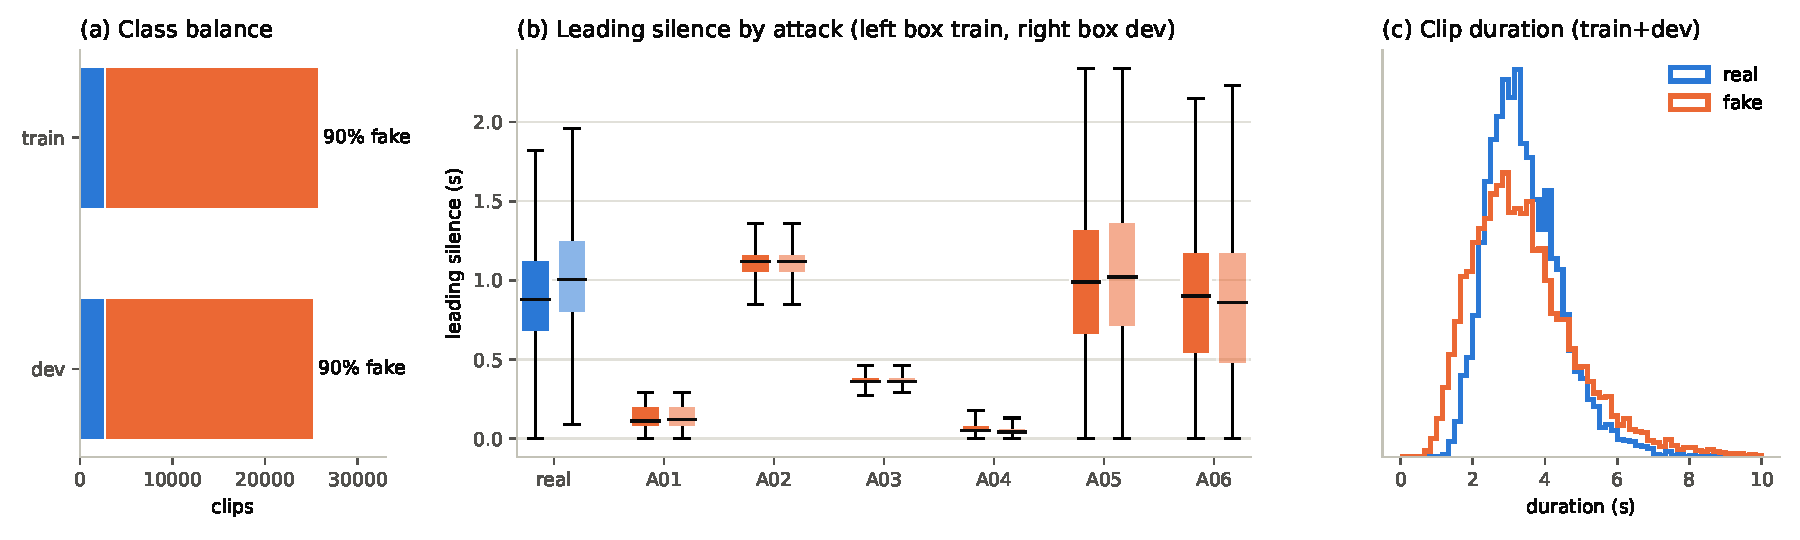
\includegraphics[width=\textwidth]{audit_silence.pdf}
\caption{Data audit (train and dev). (a) Class balance. (b) Leading silence: real vs each training
attack (left box train, right box dev). (c) Clip duration by class.}
\end{figure}
\begin{figure}[h]\centering
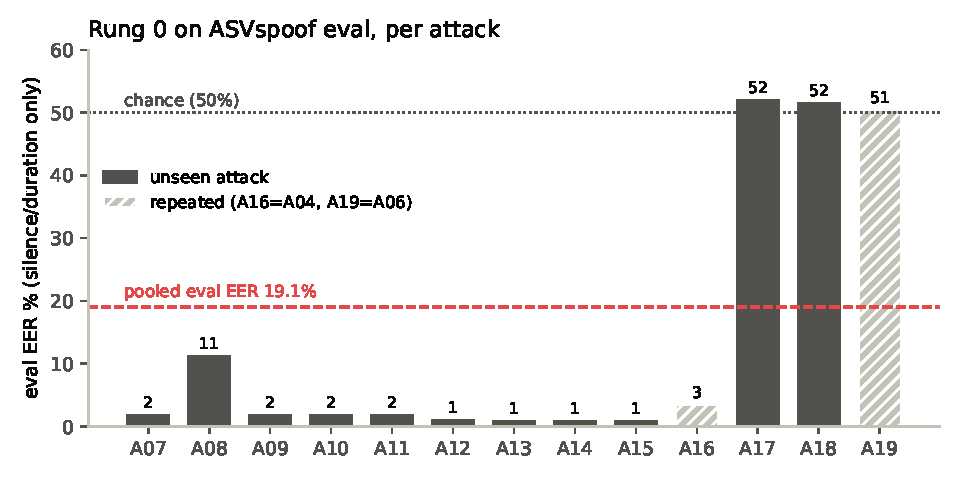
\includegraphics[width=0.56\textwidth]{rung0_eval_per_attack.pdf}\hfill
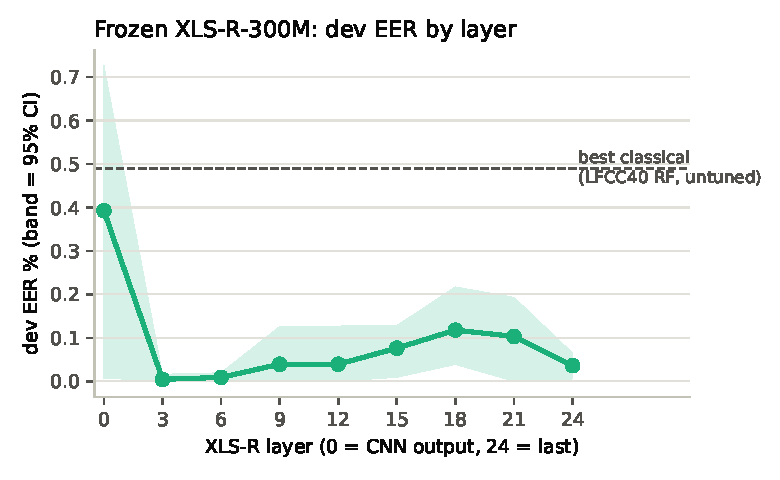
\includegraphics[width=0.42\textwidth]{xlsr_layers.pdf}
\caption{(a) Rung 0 (silence/duration only, depth-3 tree) on ASVspoof eval, per attack.
(b) Frozen XLS-R-300M: dev EER of a logistic regression on each saved layer.}
\end{figure}
\begin{figure}[h]\centering
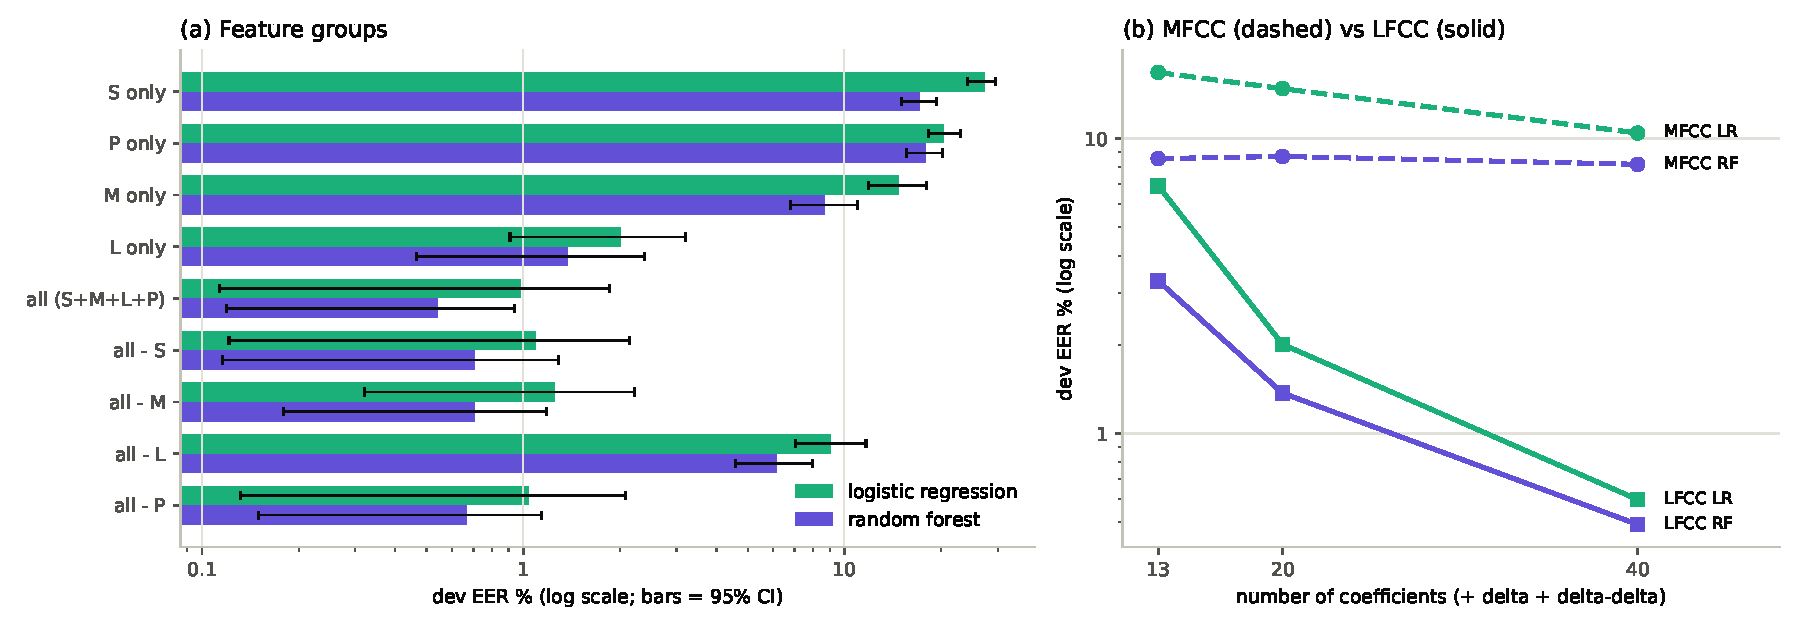
\includegraphics[width=\textwidth]{e2_features.pdf}
\caption{E2 feature ablation (dev EER, untuned). (a) Feature groups alone, all, and all-but-one.
(b) MFCC vs LFCC by number of coefficients (with $\Delta$ and $\Delta\Delta$).}
\end{figure}
\begin{figure}[h]\centering
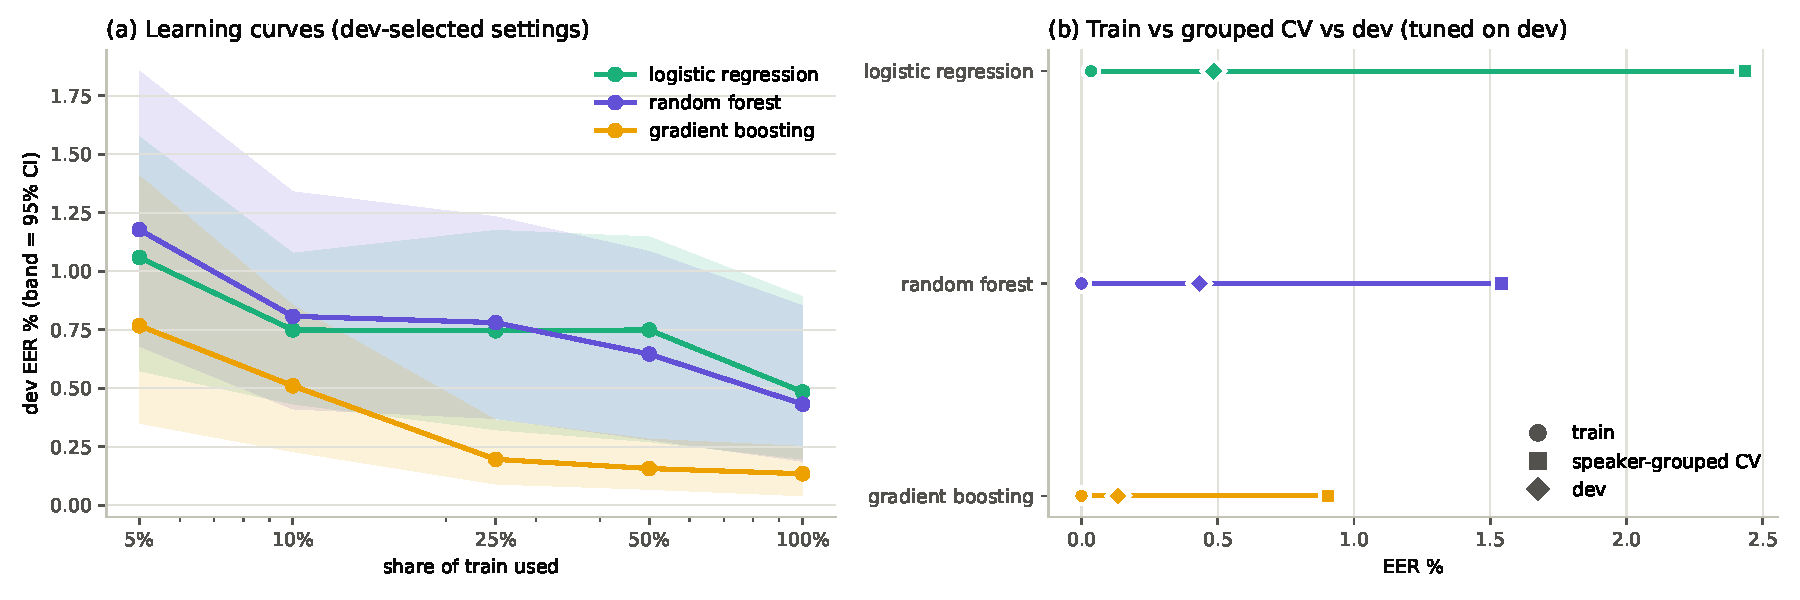
\includegraphics[width=\textwidth]{e3_tuning.pdf}
\caption{E3 on LFCC-40+$\Delta$+$\Delta\Delta$. (a) Learning curves of the dev-selected settings.
(b) Train vs speaker-grouped CV vs dev EER of the dev-selected settings.}
\end{figure}

\end{document}
